
%使用XeLaTeX编译
%版权所有,翻版必究
%本文件由程序自动生成,任何修改将被覆盖
%2019 年 01 月 23 日




\FloatBarrier
\section{
ColorOverlay
}\label{c000015s000004}


ColorOverlay用于在可渲染对象上叠加一个颜色。其常见属性
见\tablename\ \ref{tb000003}。


%使用XeLaTeX编译
%版权所有,翻版必究
%本文件由程序自动生成,任何修改将被覆盖
%2019 年 01 月 23 日



%表
\begin{longtable}{ccc}

%表头....
\toprule{}类名 
&
分类
&
简介%there must use marginnote ...
\marginnote{\setlength\fboxsep{2pt}\fbox{\footnotesize{\kaishu\tablename\,}\footnotesize{\ref{tb000000}}}}
\\ \midrule 
\endfirsthead

%表尾...
\bottomrule
\caption{ThresholdMask}\label{tb000000} 
\endlastfoot

%重复表头
\toprule{}类名 
&
分类
&
简介
\\ \midrule
\endhead
%重复表尾
\midrule
\endfoot 
Blend & aabbc & cccc \\
BrightnessContrast & aabbc & cccc \\
ColorOverlay & aabbc & cccc \\
Colorize & aabbc & cccc \\
Desaturate & aabbc & cccc \\
GammaAdjust & aabbc & cccc \\
HueSaturation & aabbc & cccc \\
LevelAdjust & aabbc & cccc \\
ConicalGradient & aabbc & cccc \\
LinearGradient & aabbc & cccc \\
RadialGradient & aabbc & cccc \\
Displace & aabbc & cccc \\
DropShadow & aabbc & cccc \\
InnerShadow & aabbc & cccc \\
FastBlur & aabbc & cccc \\
GaussianBlur & aabbc & cccc \\
MaskedBlur & aabbc & cccc \\
RecursiveBlur & aabbc & cccc \\
DirectionalBlur & aabbc & cccc \\
RadialBlur & aabbc & cccc \\
ZoomBlur & aabbc & cccc \\
Glow & aabbc & cccc \\
RectangularGlow & aabbc & cccc \\
OpacityMask & aabbc & cccc \\
ThresholdMask  & aabbc & cccc \\
\end{longtable}
%表





%使用XeLaTeX编译
%版权所有,翻版必究
%本文件由程序自动生成,任何修改将被覆盖
%2019 年 01 月 23 日






%    file:///G:/qt-everywhere-src-5.12.0/qtgraphicaleffects/src/effects/shaders/+glslcore/coloroverlay.frag


ColorOverlay的关键代码
见\filesourcenumbernameone\ \ref{f000078}。
%\begin{spacing}{1.0}
\refstepcounter{filesourcenumber}\label{f000078}    %增加源代码编号
\FloatBarrier                                  %强制完成浮动体布局
\begin{thebookfilesourceone}[escapeinside={(*@}{@*)},
caption=GoodLuck,
title=\filesourcenumbernameone \thefilesourcenumber
]
/*+glslcore/coloroverlay.frag*/
#version 150 core
in vec2 qt_TexCoord0;
uniform float qt_Opacity;
uniform sampler2D source;
uniform vec4 color;
out vec4 fragColor;
void main() {
    vec4 pixelColor = texture(source, qt_TexCoord0);
    fragColor = vec4(
        mix(pixelColor.rgb/max(pixelColor.a, 0.00390625),
            color.rgb/max(color.a, 0.00390625),
            color.a) * pixelColor.a,
        pixelColor.a) * qt_Opacity;
}(*@\marginpar[\hfill\setlength\fboxsep{2pt}\fbox{\footnotesize{\kaishu\parbox{1em}{\setlength{\baselineskip}{2pt}\filesourcenumbernameone}}\footnotesize{\thefilesourcenumber}}]{\setlength\fboxsep{2pt}\fbox{\footnotesize{\kaishu\parbox{1em}{\setlength{\baselineskip}{2pt}\filesourcenumbernameone}}\footnotesize{\thefilesourcenumber}}}@*)\end{thebookfilesourceone}          %抄录环境
\addtocounter{lstlisting}{-1}   %sub lstlisting counter ...
%\end{spacing}


本节案例源码见\filesourcenumbernameone\ \ref{f000054}。

%begin图片
\begin{figure}[htb] %浮动体 here and top ...
%there must use marginnote ...
\marginnote{\setlength\fboxsep{2pt}\fbox{\footnotesize{\kaishu\figurename\,}\footnotesize{\ref{p000020}}}}\centering %中心对齐
\setlength\fboxsep{0pt}\fcolorbox[rgb]{0,0,0}{0.97,0.98,0.99}{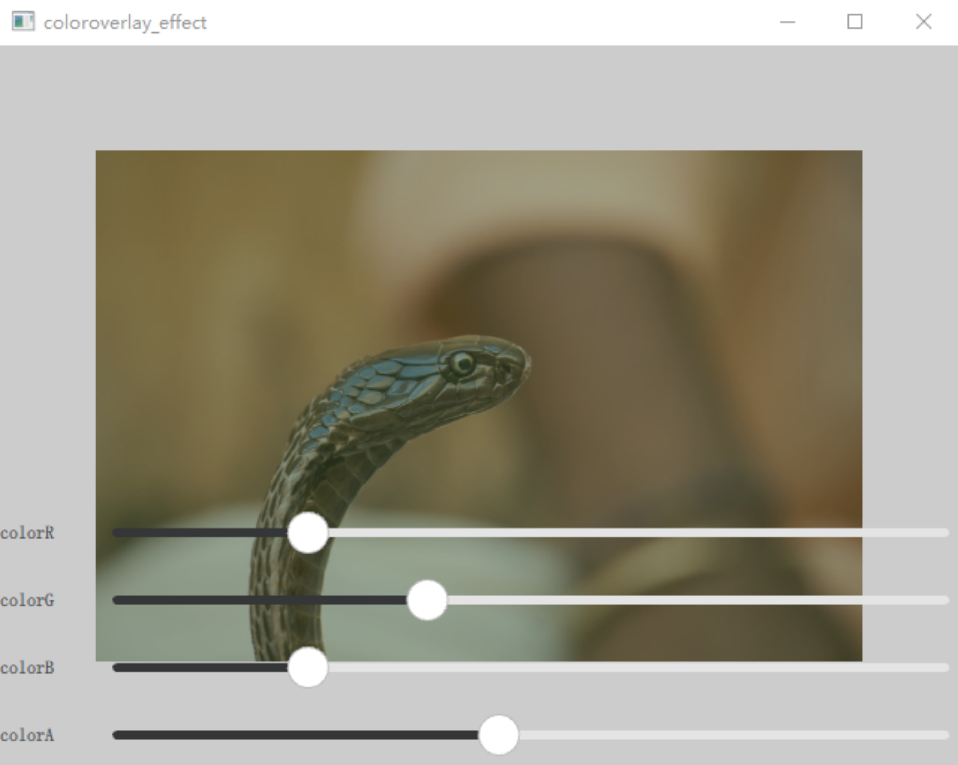
\includegraphics[width=0.95\textwidth]{the_book_image/p000020.pdf}} %图片路径
\caption{ColorOverlay} %标题
\label{p000020} %索引
\end{figure}
%end图片


%\begin{spacing}{1.0}
\refstepcounter{filesourcenumber}\label{f000054}    %增加源代码编号
\FloatBarrier                                  %强制完成浮动体布局
\begin{thebookfilesourceone}[escapeinside={(*@}{@*)},
caption=GoodLuck,
title=\filesourcenumbernameone \thefilesourcenumber
]
/*coloroverlay_effect/main.qml*/
import QtQuick 2.9
import QtGraphicalEffects 1.12

Rectangle {

    id : idRoot
    width: 640;
    height: 480;
    color: Qt.rgba(0.8,0.8,0.8,1);

    Image{
        width: parent.width * 0.8;
        height: parent.height * 0.8;
        anchors.centerIn: parent
        source: "image.jpg"
        visible: false
        fillMode: Image.PreserveAspectFit
        id : idImage
    }

    ColorOverlay{
        anchors.fill: idImage
        source: idImage
        color: idColoroverlayControl.applyColor
    }

    ColoroverlayControl{
        id : idColoroverlayControl
    }

}(*@\marginpar[\hfill\setlength\fboxsep{2pt}\fbox{\footnotesize{\kaishu\parbox{1em}{\setlength{\baselineskip}{2pt}\filesourcenumbernameone}}\footnotesize{\thefilesourcenumber}}]{\setlength\fboxsep{2pt}\fbox{\footnotesize{\kaishu\parbox{1em}{\setlength{\baselineskip}{2pt}\filesourcenumbernameone}}\footnotesize{\thefilesourcenumber}}}@*)\end{thebookfilesourceone}          %抄录环境
\addtocounter{lstlisting}{-1}   %sub lstlisting counter ...
%\end{spacing}



% ______all_key_words
% the_book_chapter the_book_subsection the_book_subsubsection
% the_book_section the_book_image the_book_table
% the_book_file the_book_tree_file the_book_command_file
% littlelongworld tabbing ref
% figurename tablename filesourcenumbernameone
% treeindexnumbernameone commandnumbernameone footnote
% item itemize comment textbullet
% \hspace*{\parindent}
% FloatBarrier







%使用XeLaTeX编译
%版权所有,翻版必究
%本文件由程序自动生成,任何修改将被覆盖
%2019 年 01 月 23 日



